\documentclass[../../main.tex]{subfiles}
\begin{document}

\subsection*{10.21}
Un campo magnetico variabile nel tempo con la legge $\vec{B} = \vec{u_n}(0.05t^2 - 0.2t)[T]$ è definito in una regione cilindrica di raggio $R = 5\ cm$; in tale regione il campo è uniforme e parallelo all'asse.\\
Calcolare la forza $F_1$ cha agisce su un elettrone (fermo) a distanza $r_1 = 0.04\ m$ dal centro dell'asse all'istante $t_1 = 4\ s$.\\
Calcolare la forza $F_2$ che agisce nello stesso istante a una distanza $r_2 = 0.07\ m$ dal centro.\\
Calcolare l'istante in cui a qualsiasi distanza la forza è nulla.\\
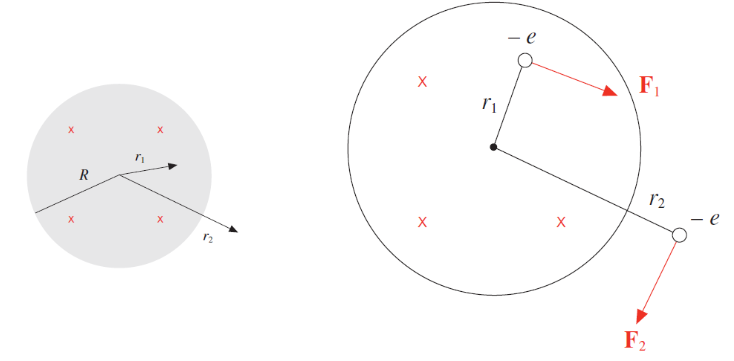
\includegraphics[scale=0.3]{e_10_21.png}
\subsubsection*{Formule utilizzate}
\subsubsection*{Soluzione punto a}
Il campo magnetico dipende dal tempo B(t) produce un campo elettrico E(t) anche dipendente dal tempo secondo la legge:\\
$\varepsilon_i = \oint\vec{E}(t)d\vec{s}=-\frac{d\Phi(\vec{B}(t))}{dt} = -\frac{d}{dt}\int_\Sigma \vec{B}\vec{u_n}d\Sigma$\\
Per $0\le r\le R$:\\
$-\frac{d\Phi(\vec{B}(t))}{dt} = -\pi r^2\frac{dB}{dt}=-\pi r^2(0.1t - 0.2)$\\
$\varepsilon_i = \oint \vec{E}(t)d\vec{s} = 2\pi rE$\\
Eguagliando i due risultati: $-\pi r^2(01.t-0.2) = 2\pi rE$\\
da cui: $E = -\frac{r}{2} (0.1t-0.2)$ con segno +, cioè in senso antiorario.\\
Ovvero $\vec{E}$ circola in verso antiorario fino a $t = 2\ s$ e poi in verso orario.
$F_1 = qE_1 = 6.4 * 10^{-22}\ N$ (verso antiorario)\\
\subsubsection*{Soluzione punto b}
Per $r \ge R$:
$\Phi(\vec{B}) = \int_\Sigma\vec{B}\vec{u_n}d\Sigma = B\pi R^2$\\
$-\frac{d\Phi(\vec{B}(t))}{dt} = -\pi R^2\frac{dB}{dt} = -\pi R^2(0.1t-0.2)$\\
$varepsilon_i = \oint \vec{E}(t)d\vec{s} = 2\pi rE$.\\
Uguagliando i risulati otteniamo:\\
$E = -\frac{R^2}{2r}(0.1t-0.2)$\\
$F_2 = qE_2 = e\frac{R^2}{2r_2}(0.1t_1 -0.2) =5.7* 10^{-22}\ N$ anche in questo caso in senso antiorario.\\
\subsubsection*{Soluzione punto c}
Siccome a qualsiasi distanza la forza è proporzionale a (0.1t -0.2) la forza diventa nulla quando:\\
$0.1t-0.2 = 0$\tab\tab $F=0$ per $t=2\ s$\\
Questo corrisponde al tempo in corrispondenza al quale il campo magnetico assume il suo valore minimo pari a $-0.2\ T$.
\newpage

\end{document}